% Espansione Teorica per Git - DAG e Architettura Interna
% Da integrare nel capitolo 01_introduzione_git.tex

\section{Git come Directed Acyclic Graph (DAG)}

\subsection{Teoria dei Grafi Applicata a Git}

\begin{tcolorbox}[colback=blue!10, colframe=blue!60, title=Definizione: DAG in Git]
La storia di Git è un \textbf{Grafo Aciclico Diretto (DAG)} dove:

\begin{itemize}
    \item \textbf{Nodi}: Commit (snapshot del progetto)
    \item \textbf{Archi diretti}: Relazioni parent → child
    \item \textbf{Aciclico}: Nessun ciclo (tempo unidirezionale)
\end{itemize}

\textbf{Formalmente}:
\[
G = (V, E) \quad \text{dove} \quad V = \{\text{commits}\}, \quad E \subseteq V \times V
\]

Proprietà: $\forall v \in V: \nexists$ cammino da $v$ a $v$
\end{tcolorbox}

\textbf{Rappresentazione Visuale}:

\begin{figure}[h]
\centering
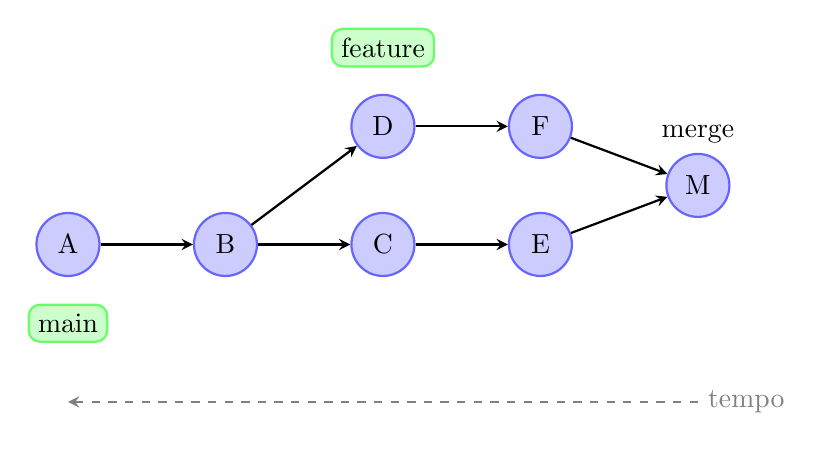
\begin{tikzpicture}[
    commit/.style={circle, draw=blue!60, fill=blue!20, thick, minimum size=8mm},
    branch/.style={rectangle, draw=green!60, fill=green!20, rounded corners},
    ->, >=stealth, thick
]
    % Commits
    \node[commit] (c1) at (0,0) {A};
    \node[commit] (c2) at (2,0) {B};
    \node[commit] (c3) at (4,0) {C};
    \node[commit] (c4) at (4,1.5) {D};
    \node[commit] (c5) at (6,0) {E};
    \node[commit] (c6) at (6,1.5) {F};
    \node[commit] (c7) at (8,0.75) {M};

    % Edges
    \draw[->] (c1) -- (c2);
    \draw[->] (c2) -- (c3);
    \draw[->] (c2) -- (c4);
    \draw[->] (c3) -- (c5);
    \draw[->] (c4) -- (c6);
    \draw[->] (c5) -- (c7);
    \draw[->] (c6) -- (c7);

    % Labels
    \node[branch] at (0,-1) {main};
    \node[branch] at (4,2.5) {feature};
    \node[above] at (c7.north) {merge};

    % Time arrow
    \draw[<-, dashed, gray] (0,-2) -- (8,-2) node[right] {tempo};
\end{tikzpicture}
\caption{Git DAG con branch e merge}
\end{figure}

\subsection{Operazioni su DAG: Complessità}

\begin{table}[h]
\centering
\begin{tabular}{|l|c|p{6cm}|}
\hline
\textbf{Operazione} & \textbf{Complessità} & \textbf{Algoritmo} \\
\hline
\hline
\texttt{git log} & $O(V + E)$ & DFS traversal dal HEAD \\
\hline
\texttt{git merge-base A B} & $O(V + E)$ & Lowest Common Ancestor (LCA) \\
\hline
\texttt{git rebase} & $O(n \log n)$ & Re-apply commits + sort \\
\hline
\texttt{git cherry-pick} & $O(1)$ & Single commit apply \\
\hline
\texttt{git bisect} & $O(\log V)$ & Binary search su DAG \\
\hline
\texttt{git blame} & $O(V \cdot L)$ & Annotation per line \\
\hline
\end{tabular}
\caption{Complessità operazioni Git}
\end{table}

\subsection{Architettura Interna: Content-Addressable Filesystem}

\begin{tcolorbox}[colback=green!10, colframe=green!60, title=Git Object Model]
Git memorizza tutto come \textbf{oggetti immutabili} identificati da hash SHA-1 (160 bit):

\[
\text{hash} = \text{SHA-1}(\text{header} + \text{content})
\]

\textbf{Tipi di oggetti}:

\begin{enumerate}
    \item \textbf{Blob}: Contenuto file
    \begin{lstlisting}
blob 14\0Hello, world!
SHA-1: a0423896973644771497bdc03eb99d5281615b51
    \end{lstlisting}

    \item \textbf{Tree}: Directory structure
    \begin{lstlisting}
tree 72\0
100644 blob a042... README.md
040000 tree b719... src/
    \end{lstlisting}

    \item \textbf{Commit}: Snapshot + metadata
    \begin{lstlisting}
commit 234\0
tree b719...
parent c3d8...
author Name <email> 1699876543 +0100
committer Name <email> 1699876543 +0100

Commit message
    \end{lstlisting}

    \item \textbf{Tag}: Riferimento annotato
\end{enumerate}
\end{tcolorbox}

\textbf{Deduplicazione Automatica}:

File identici → stesso hash → unico blob memorizzato

\begin{lstlisting}[caption=Risparmio Spazio con Deduplicazione]
# 1000 file identici da 10KB
Senza Git: 1000 × 10KB = 10MB
Con Git: 1 blob + 1000 ref = 10KB + overhead

Risparmio: ~99.9%!
\end{lstlisting}

\section*{Conclusione}

Git è fondato su solide basi teoriche:
\begin{itemize}
    \item \textbf{DAG}: Storia come grafo aciclico
    \item \textbf{Hash-based}: Content-addressable filesystem
    \item \textbf{Immutabilità}: Oggetti mai modificati
    \item \textbf{Efficienza}: Operazioni $O(\log n)$ o $O(n)$
\end{itemize}
